\chapter{Óptica geométrica: rayos, reflexión, refracción}\label{ch:b1:rays-reflection-refraction}

Una pajita metida en un vaso de agua parece quebrada en la superficie; un
nadador que mira hacia arriba desde el fondo de una piscina ve el cielo
entero comprimido en un disco brillante, rodeado por un espejo del suelo
de la piscina; una fibra de vidrio del grosor de un cabello lleva una
llamada telefónica de un lado a otro de un océano con menos pérdidas que
las que sufre un hilo de cobre al cruzar una calle. Tres leyes --- la luz
se propaga en línea recta, se refleja con ángulos iguales, se desvía según
la regla de Snell --- dan cuenta de todo ello; este capítulo las enuncia
con precisión, señala dónde dejan de ser ciertas y las pone a trabajar.

\begin{omfigure}
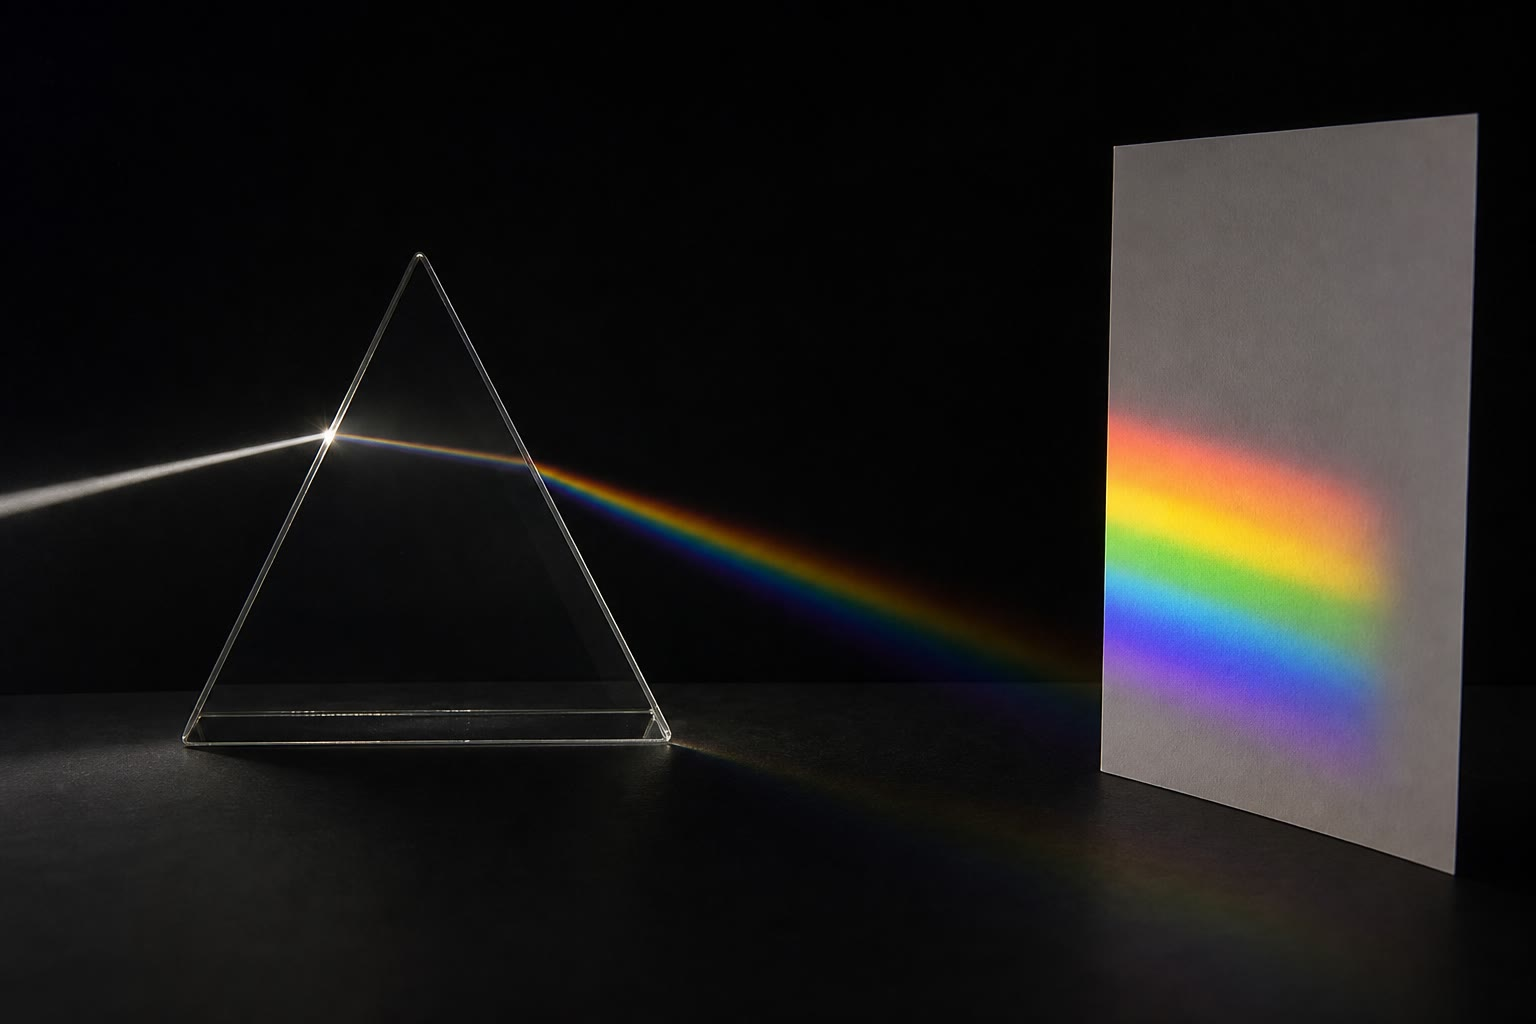
\includegraphics[width=0.58\linewidth]{images/book3/ai/b3-02-prism-dispersion-v2.jpg}

{\small Un prisma desvía un haz blanco hacia su base y lo despliega: el índice del vidrio depende de la longitud de onda, y el violeta es el más desviado.}
\end{omfigure}

\section{El modelo de la óptica geométrica}

\begin{definition}[Rayo luminoso; medio homogéneo]\label{def:b1:rays-reflection-refraction:ray}
\index{rayo luminoso}\index{óptica geométrica}\index{medio homogéneo}
En el modelo de la \emph{óptica geométrica}, la luz se propaga a lo largo
de \emph{rayos luminosos}: curvas orientadas que son rectas en un medio
\emph{homogéneo} (con las mismas propiedades en todos sus puntos) y que
transportan energía con independencia unas de otras. Un haz es un manojo
de rayos; una fuente puntual emite rayos en todas las direcciones.
\end{definition}

\begin{definition}[Índice de refracción]\label{def:b1:rays-reflection-refraction:index}
\index{índice de refracción}\index{medio transparente}
Un medio \emph{transparente} deja pasar la luz; la luz se propaga en él a
una velocidad $v < c$. Su \emph{índice de refracción} es
\[
n = \frac{c}{v} \geq 1 .
\]
Vacío: $n = 1$; aire: $1.0003$; agua: $1.33$; vidrio ordinario: de $1.5$
a $1.6$; diamante: $2.42$. Una onda de frecuencia $\nu$ conserva su
frecuencia al entrar en un medio, de modo que su longitud de onda pasa de $\lambda_0 =
c/\nu$ en el vacío a $\lambda = \lambda_0/n$.
\end{definition}

\begin{remark}[Dispersión]\label{rem:b1:rays-reflection-refraction:dispersion}
\index{dispersión (óptica)}\index{ley de Cauchy}
En la materia el índice depende ligeramente de la longitud de onda: el
medio es \emph{dispersivo}. Para el vidrio en el visible, la ley empírica
de Cauchy $n(\lambda) = A + B/\lambda^2$ se ajusta bien: $n$ es mayor para
el azul que para el rojo en unos $0.01$ o $0.02$. El prisma y el \omterm{ex:b1:rays-reflection-refraction:rainbow}{arco
iris}, al final de este capítulo, viven de esa diferencia.
\end{remark}

\begin{remark}[Límites del modelo]\label{rem:b1:rays-reflection-refraction:limits}
La luz es una onda, y una onda que atraviesa una abertura de anchura $a$
se abre en un ángulo del orden de $\lambda/a$ (difracción,
\cref{ch:b1:wave-propagation}). Los rayos son una buena descripción
mientras toda abertura, lente y obstáculo sea mucho mayor que la longitud
de onda (de \qty{0.4}{} a \qty{0.8}{\micro m} para la luz visible): un
agujero de \qty{1}{mm} abre un haz en $10^{-3}$ radianes, despreciable
sobre una mesa de trabajo; uno de \qty{1}{\micro m} lo reparte por todo el
semiespacio y ninguna imagen de rayos sobrevive. El \omterm{def:b1:rays-reflection-refraction:fiber}{núcleo} de
\qty{9}{\micro m} de una fibra monomodo de telecomunicaciones ya está
fuera del modelo.
\end{remark}

\begin{proposition}[Retorno inverso de la luz]\label{prop:b1:rays-reflection-refraction:reversibility}
\index{principio del retorno inverso}
El trayecto de un rayo no depende del sentido en que la luz lo recorre:
si la luz va de $A$ a $B$ por un camino, la luz que parte de $B$ sigue el
mismo camino hasta $A$.
\end{proposition}
\admitted

\section{Reflexión y refracción}

\begin{definition}[Incidencia]\label{def:b1:rays-reflection-refraction:incidence}
\index{plano de incidencia}\index{ángulo de incidencia}\index{dioptrio}
Un rayo que alcanza en un punto $I$ la superficie que separa dos medios
(un \emph{dioptrio}) forma con la \emph{normal} a la superficie en $I$ el
\emph{ángulo de incidencia} $i_1$. El \emph{plano de incidencia} contiene
al rayo incidente y a la normal.
\end{definition}

\begin{theorem}[Leyes de la reflexión y de la refracción (Snell--Descartes)]\label{thm:b1:rays-reflection-refraction:snell}
\index{reflexión!ley de la}\index{refracción!ley de la}\index{ley de Snell}
En la superficie que separa medios de índices $n_1$ (lado incidente) y
$n_2$:
\begin{enumerate}
  \item los rayos reflejado y refractado están en el \omterm{def:b1:rays-reflection-refraction:incidence}{plano de incidencia};
  \item el rayo reflejado forma con la normal el ángulo $i_1' = i_1$,
        al otro lado de la normal;
  \item el rayo refractado forma con la normal un ángulo $i_2$ tal que
        \[
        n_1 \sin i_1 = n_2 \sin i_2 .
        \]
\end{enumerate}
\end{theorem}
\admitted

\begin{remark}[De dónde vienen las leyes]\label{rem:b1:rays-reflection-refraction:fermat}
\index{principio de Fermat}
Las dos leyes se siguen del \emph{\omterm{rem:b1:rays-reflection-refraction:fermat}{principio de Fermat}}: entre dos puntos,
la luz sigue el camino de menor tiempo de recorrido. La reflexión con
ángulos iguales es el camino quebrado más corto que toca el espejo; la \omterm{thm:b1:rays-reflection-refraction:snell}{ley
de Snell} es el camino que compensa un trayecto más largo en el medio
rápido con uno más corto en el medio lento
(\cref{exo:b1:rays-reflection-refraction:12}). En el volumen del Año 2
ambas leyes se deducen de la naturaleza ondulatoria de la luz en una
interfaz.
\end{remark}

\begin{omfigure}
\begin{tikzpicture}[font=\small, x=1cm, y=1cm]
  \fill[omDef!10] (-3.6,-2.4) rectangle (3.6,0);
  \draw[thick] (-3.6,0) -- (3.6,0);
  \draw[dashed] (0,-2.4) -- (0,2.6) node[above] {normal};
  \node at (-3.0,0.4) {$n_1$};
  \node at (-2.85,-0.45) {$n_2 > n_1$};
  % incident at 50 deg from normal
  \draw[-Stealth, omThm, thick] (-2.3,1.93) -- (-1.15,0.965);
  \draw[omThm, thick] (-1.15,0.965) -- (0,0);
  % reflected
  \draw[omThm, thick] (0,0) -- (1.15,0.965);
  \draw[-Stealth, omThm, thick] (1.15,0.965) -- (2.3,1.93);
  % refracted at 31 deg
  \draw[omDef, thick] (0,0) -- (0.62,-1.03);
  \draw[-Stealth, omDef, thick] (0.62,-1.03) -- (1.24,-2.06);
  \draw (0,1.1) arc (90:140:1.1); \node at (-0.5,1.4) {$i_1$};
  \draw (0,1.1) arc (90:40:1.1); \node at (0.5,1.4) {$i_1'$};
  \draw (0,-1.1) arc (270:301:1.1); \node at (0.45,-1.45) {$i_2$};
  \fill (0,0) circle (1.2pt); \node[above left, xshift=-2pt] at (0,0) {$I$};
\end{tikzpicture}

{\small Reflexión y refracción en la superficie que separa dos medios.
El rayo refractado se acerca a la normal cuando $n_2 > n_1$; los tres
rayos y la normal están en un mismo plano, el plano de la figura.}
\end{omfigure}

\begin{proposition}[Hacia dónde se desvía el rayo]\label{prop:b1:rays-reflection-refraction:bending}
Al entrar en un medio más refringente ($n_2 > n_1$), un rayo se desvía
\emph{acercándose} a la normal ($i_2 < i_1$); al entrar en uno menos
refringente, \emph{alejándose} de ella ($i_2 > i_1$). Un rayo que sigue la
normal la atraviesa sin desviarse.
\end{proposition}

\begin{proof}
$\sin i_2 = (n_1/n_2)\sin i_1$, con $\sin$ creciente en
$[0, \pi/2]$.
\end{proof}

\begin{example}[Profundidad aparente]\label{ex:b1:rays-reflection-refraction:depth}
\index{profundidad aparente}
Una moneda descansa a profundidad $h$ bajo el agua ($n = 1.33$), vista
casi desde la vertical. Un rayo que sale de la moneda y llega a la
superficie con un ángulo pequeño $i_2$ (en el agua) emerge con $i_1$ tal
que $\sin i_1 = n\sin i_2$; para ángulos pequeños, $i_1 \approx n\,i_2$. El
ojo prolonga hacia atrás el rayo emergente: parece proceder de una
profundidad $h'$ con $\tan i_1 \approx x/h'$ y $\tan i_2 \approx x/h$ para
el mismo punto de la superficie, situado a distancia $x$ de la vertical,
de modo que $h' = h\,i_2/i_1 = h/n$. Una piscina de \qty{2.0}{m} de fondo
parece de \qty{1.5}{m}; un pez ve al pescador $1.33$ veces más alto de lo
que está.
\end{example}

\begin{theorem}[Reflexión total]\label{thm:b1:rays-reflection-refraction:tir}
\index{reflexión total}\index{ángulo límite}
La luz que va de un medio de índice $n_1$ hacia otro menos refringente
($n_2 < n_1$) solo se refracta si $i_1 \leq i_c$, donde el
\emph{\omterm{thm:b1:rays-reflection-refraction:tir}{ángulo límite}} cumple
\[
\sin i_c = \frac{n_2}{n_1} .
\]
Para $i_1 > i_c$ no hay rayo refractado: la superficie refleja toda la
luz --- es la \emph{\omterm{thm:b1:rays-reflection-refraction:tir}{reflexión total}}.
\end{theorem}

\begin{proof}
La \omterm{thm:b1:rays-reflection-refraction:snell}{ley de Snell} exige $\sin i_2 = (n_1/n_2)\sin i_1 > \sin i_1$; esto
supera $1$ en cuanto $\sin i_1 > n_2/n_1$, y entonces no existe ningún
ángulo $i_2$. Para $i_1 = i_c$ el rayo refractado sale rasante a la
superficie ($i_2 = 90^\circ$). Que \emph{toda} la energía se refleje
entonces es un enunciado sobre intensidades, del que la \omterm{def:b1:rays-reflection-refraction:ray}{óptica geométrica}
no se ocupa; el tratamiento ondulatorio del volumen del Año 2 lo confirma.
\end{proof}

\begin{omfigure}
\begin{tikzpicture}[font=\small, x=1cm, y=1cm]
  \fill[omDef!10] (-4.2,-2.2) rectangle (4.2,0);
  \draw[thick] (-4.2,0) -- (4.2,0);
  \node at (3.0,0.85) {aire $n_2 = 1$};
  \node at (2.9,-0.55) {agua $n_1 = 1.33$};
  \fill (-3,-2) circle (1.5pt) node[below] {$S$};
  % ray 1: i1 = 30 deg -> hits surface at x = -3 + 2 tan30 = -1.845 ; refracted i2 = 41.7
  \draw[-Stealth, omThm, thick] (-3,-2) -- (-1.845,0);
  \draw[-Stealth, omThm, thick] (-1.845,0) -- ++(41.7:1.6);
  % ray 2: i1 = 48.8 (critical): hits at x = -3 + 2 tan48.8 = -0.716 ; refracted grazing
  \draw[-Stealth, omProp, thick] (-3,-2) -- (-0.716,0);
  \draw[-Stealth, omProp, thick] (-0.716,0) -- (1.3,0.02);
  \draw[omProp, thick] (-0.716,0) -- ++(131.2:1.5);
  % ray 3: i1 = 65: hits at x = -3 + 2 tan65 = 1.289 ; totally reflected
  \draw[-Stealth, omDef!70!black, thick] (-3,-2) -- (1.289,0);
  \draw[-Stealth, omDef!70!black, thick] (1.289,0) -- ++(115:2.1);
  \draw[dashed] (-1.845,-1.0) -- (-1.845,1.0);
  \draw (-1.845,-0.6) arc (270:240:0.6); \node at (-2.2,-0.85) {$i_1$};
  \node[omThm] at (-1.55,1.35) {\footnotesize refractado};
  \node[omProp, right] at (1.45,0.3) {\footnotesize rasante, $i_1 = i_c$};
  \node[omDef!70!black] at (1.55,2.05) {\footnotesize solo reflejado};
\end{tikzpicture}

{\small Rayos procedentes de una fuente $S$ bajo el agua. Por debajo del
\omterm{thm:b1:rays-reflection-refraction:tir}{ángulo límite} ($i_c = 48.8^\circ$ para agua--aire) parte de la luz sale;
en $i_c$ el rayo refractado sale rasante; más allá, la superficie es un
espejo perfecto --- el disco brillante de cielo del nadador tiene ese
ángulo por frontera.}
\end{omfigure}

\begin{example}[Diamantes y nadadores]\label{ex:b1:rays-reflection-refraction:tir}
Vidrio--aire: $\sin i_c = 1/1.5$, $i_c = 41.8^\circ$, y por eso un prisma
de $45^\circ$ refleja totalmente y sustituye a un espejo en unos
prismáticos. Diamante--aire: $i_c = 24.4^\circ$; un diamante tallado
atrapa la luz que entra por su cara superior y la devuelve casi entera por
esa misma cara --- el brillo es \omterm{thm:b1:rays-reflection-refraction:tir}{reflexión total}, el fuego es dispersión.
Agua--aire: $i_c = 48.8^\circ$; al mirar hacia arriba, un buceador ve el
cielo entero dentro de un cono de semiángulo $48.8^\circ$ (la ``ventana de
Snell'') y, fuera de él, el fondo reflejado.
\end{example}

\section{La fibra óptica}

\begin{definition}[Fibra de índice escalonado]\label{def:b1:rays-reflection-refraction:fiber}
\index{fibra óptica}\index{núcleo}\index{revestimiento}\index{apertura numérica}
Una \emph{fibra óptica de índice escalonado} es un \emph{núcleo}
cilíndrico de vidrio de índice $n_1$ envuelto en un \emph{revestimiento}
de índice $n_2$ ligeramente menor. La luz que entra en el núcleo dentro de
un cono de semiángulo $\theta_a$ en torno al eje queda guiada por
reflexiones totales sucesivas en la superficie núcleo--revestimiento. La
\emph{apertura numérica} es $\mathrm{NA} = \sin\theta_a$.
\end{definition}

\begin{proposition}[Cono de aceptación y ensanchamiento intermodal]\label{prop:b1:rays-reflection-refraction:fiber}
\index{ángulo de aceptación}\index{dispersión intermodal}
Para una fibra cuya cara de entrada está en el aire,
\[
\sin\theta_a = \sqrt{n_1^2 - n_2^2} .
\]
A lo largo de una longitud $L$, el rayo guiado paralelo al eje y el rayo
guiado más inclinado llegan con un retraso
\[
\Delta t = \frac{L\,n_1}{c}\left(\frac{n_1}{n_2} - 1\right)
\]
entre ellos (\emph{\omterm{prop:b1:rays-reflection-refraction:fiber}{dispersión intermodal}}).
\end{proposition}

\begin{proof}
Un rayo que entra formando un ángulo $\theta$ con el eje se refracta a
$\theta'$ con $\sin\theta = n_1\sin\theta'$ y alcanza el \omterm{def:b1:rays-reflection-refraction:fiber}{revestimiento} con
incidencia $i = 90^\circ - \theta'$. El guiado exige $\sin i \geq n_2/n_1$,
es decir $\cos\theta' \geq n_2/n_1$, es decir $\sin\theta' \leq
\sqrt{1 - n_2^2/n_1^2}$; basta multiplicar por $n_1$. El rayo axial
recorre $L$ a velocidad $c/n_1$: $t_0 = Ln_1/c$. El rayo más inclinado
zigzaguea con ángulo $\theta'_{\max}$ tal que $\cos\theta'_{\max} = n_2/n_1$;
su camino mide $L/\cos\theta'_{\max} = L n_1/n_2$, luego
$t_1 = L n_1^2/(n_2 c)$, y $\Delta t = t_1 - t_0$.
\end{proof}

\begin{omfigure}
\begin{tikzpicture}[font=\small, x=1cm, y=1cm]
  \fill[omDef!6] (0,-1.0) rectangle (7.8,1.0);
  \fill[omDef!18] (0,-0.55) rectangle (7.8,0.55);
  \draw (0,0.55) -- (7.8,0.55); \draw (0,-0.55) -- (7.8,-0.55);
  \draw (0,1.0) -- (7.8,1.0); \draw (0,-1.0) -- (7.8,-1.0);
  \draw[thick] (0,-1.0) -- (0,1.0);
  \draw[dashed] (-0.2,0) -- (7.8,0);
  \node[right] at (7.8,0.78) {revestimiento $n_2$};
  \node[right] at (7.8,0) {núcleo $n_1$};
  \node[right] at (7.8,-0.78) {revestimiento $n_2$};
  % entering ray at theta_a = 25 deg for drawing, refracted to 16 deg
  \draw[-Stealth, omThm, thick] (-1.6,-0.746) -- (0,0);
  \draw[omThm, thick] (0,0) -- (1.92,0.55) -- (5.76,-0.55) -- (7.8,0.035);
  \draw[-Stealth, omThm, thick] (7.0,-0.194) -- (7.8,0.035);
  \draw[dashed] (1.92,1.3) -- (1.92,-0.2);
  \draw (1.92,0.55) ++(0,0.5) arc (90:164:0.5); \node at (1.45,1.2) {$i$};
  \draw[omThm!50, dashed] (-1.6,0.746) -- (0,0);
  \draw (-0.9,0) arc (180:205:0.9); \node at (-1.25,-0.28) {$\theta_a$};
  \draw[omDef!70!black, thick] (0,0) -- (7.8,0);
  \draw (0.9,0) arc (0:16:0.9); \node at (1.2,0.15) {$\theta'$};
  \node[omDef!70!black, below] at (4.0,-1.05) {rayo axial: camino más corto, llega el primero};
\end{tikzpicture}

{\small Una fibra de índice escalonado. Un rayo que entra dentro del cono
de aceptación de semiángulo $\theta_a$ alcanza el \omterm{def:b1:rays-reflection-refraction:fiber}{revestimiento} con
incidencia $i \geq i_c$ y queda guiado por reflexiones totales; el rayo
axial sigue el camino más corto y el rayo guiado más inclinado el más
largo --- un pulso se ensancha en el tiempo.}
\end{omfigure}

\begin{example}[Las cifras de una fibra de telecomunicaciones]\label{ex:b1:rays-reflection-refraction:fibernum}
$n_1 = 1.480$, $n_2 = 1.465$: $\mathrm{NA} = \sqrt{2.190 - 2.146} =
0.21$, $\theta_a = 12^\circ$; $i_c = 81.8^\circ$, de modo que los rayos
guiados no se apartan más de $8.2^\circ$ del eje. Ensanchamiento
intermodal: $\Delta t/L =
(1.48/c)(1.48/1.465 - 1) = \qty{51}{ns/km}$. En
\qty{2}{km} un pulso se ensancha \qty{0.1}{\micro s}, lo que limita el
caudal binario a unos \qty{5}{Mbit/s}: el problema de fin de semana sigue
esta limitación hasta su remedio, la fibra monomodo.
\end{example}

\section{El espejo plano}

\begin{proposition}[Imagen en un espejo plano]\label{prop:b1:rays-reflection-refraction:mirror}
\index{espejo plano}\index{imagen virtual}\index{estigmatismo}
Todos los rayos procedentes de un punto $A$ y reflejados por un \omterm{prop:b1:rays-reflection-refraction:mirror}{espejo
plano} parecen venir del punto $A'$ simétrico de $A$ respecto del plano del
espejo: $A'$ es la \emph{imagen} de $A$. Es \emph{virtual} (no pasa luz
por ella) y el espejo es \emph{rigurosamente estigmático}: todo punto
tiene una imagen puntual exacta.
\end{proposition}

\begin{proof}
Un rayo que sale de $A$ y llega al espejo en $I$ con incidencia $i$ parte
con la misma $i$ al otro lado de la normal. La recta reflejada y la normal
en $I$ forman el ángulo $i$, igual que la recta $IA$; por simetría
respecto del plano del espejo, la recta reflejada es la simétrica de la
recta $IA$ y pasa, por tanto, por el punto simétrico $A'$ --- y esto para
todo $I$.
\end{proof}

\begin{proposition}[Giro de un espejo]\label{prop:b1:rays-reflection-refraction:rotation}
Girar un \omterm{prop:b1:rays-reflection-refraction:mirror}{espejo plano} un ángulo $\alpha$ alrededor de un eje contenido en
su plano y perpendicular al \omterm{def:b1:rays-reflection-refraction:incidence}{plano de incidencia} gira el rayo reflejado un
ángulo $2\alpha$.
\end{proposition}

\begin{proof}
La normal gira $\alpha$, así que la incidencia pasa de $i$ a
$i + \alpha$; el rayo reflejado, a $i + \alpha$ al otro lado de la nueva
normal, se ha desplazado $\alpha$ (normal) $+ \alpha$ (ángulo) $=
2\alpha$ respecto de su dirección anterior.
\end{proof}

\begin{example}[La palanca del galvanómetro]\label{ex:b1:rays-reflection-refraction:galvanometer}
Un espejito pegado a la bobina de un galvanómetro, iluminado por una
lámpara y que proyecta una mancha sobre una escala a \qty{2}{m}: un giro
de $\qty{1}{mrad}$ de la bobina desplaza la mancha $2 \times 10^{-3} \times
\qty{2}{m} = \qty{4}{mm}$ --- una palanca óptica que amplifica sin
rozamiento, el principio del galvanómetro de espejo y del escáner láser.
\end{example}

\section{El prisma}

\begin{proposition}[Fórmulas del prisma]\label{prop:b1:rays-reflection-refraction:prism}
\index{prisma}\index{desviación}\index{desviación mínima}
Un rayo que atraviesa un prisma de ángulo $A$ e índice $n$ en el aire, en
el plano perpendicular a la arista, con ángulos $i$ (entrada), $r$, $r'$
(interiores) e $i'$ (salida) medidos desde las normales, cumple
\[
\sin i = n \sin r, \qquad r + r' = A, \qquad \sin i' = n \sin r',
\]
y resulta desviado en $D = i + i' - A$. La desviación es mínima cuando el
trayecto es simétrico, $i = i'$, $r = r' = A/2$; entonces
\[
n = \frac{\sin\frac{A + D_{\min}}{2}}{\sin\frac{A}{2}} .
\]
\end{proposition}

\begin{proof}
La \omterm{thm:b1:rays-reflection-refraction:snell}{ley de Snell} en cada cara; $r + r' = A$ porque las dos normales forman
el ángulo $A$ (véase el cuadrilátero que determinan la arista, los dos
puntos de incidencia y el corte de las normales). La desviación total vale
$(i - r) + (i' - r') = i + i' - A$. Por el retorno inverso de la luz, la
desviación es la misma función de $i$ que de $i'$; si el mínimo se
alcanzara en $i_0 \neq i_0'$, se alcanzaría también en la incidencia
invertida $i_0'$, y habría dos mínimos, cosa que la monotonía de $D(i)$ a
cada lado de su mínimo prohíbe: el mínimo está en $i = i'$. Entonces
$r = r' = A/2$ y $D_{\min} = 2i - A$; sustituir $i = (A +
D_{\min})/2$ en $\sin i = n\sin(A/2)$ da la fórmula.
\end{proof}

\begin{omfigure}
\begin{tikzpicture}[font=\small, x=1cm, y=1cm]
  % prism apex at top, A = 60 deg
  \coordinate (S) at (0,3.2); \coordinate (B1) at (-1.85,0); \coordinate (B2) at (1.85,0);
  \fill[omDef!10] (S) -- (B1) -- (B2) -- cycle;
  \draw[thick] (S) -- (B1) -- (B2) -- cycle;
  \node[above] at (S) {$A$};
  % entry point on left face at height 1.4: left face from (0,3.2) to (-1.85,0); param t: point = S + t*(B1-S)
  \coordinate (I) at (-1.04,1.4);
  \coordinate (J) at (1.04,1.4);
  % normals: left face direction (-1.85,-3.2) normalized; outward normal for left face points to (-3.2,1.85)/3.7 = (-0.865,0.5)
  \draw[dashed] ($(I)+(-0.865*1.3,0.5*1.3)$) -- ($(I)+(0.865*1.2,-0.5*1.2)$);
  \draw[dashed] ($(J)+(0.865*1.3,0.5*1.3)$) -- ($(J)+(-0.865*1.2,-0.5*1.2)$);
  % incident ray at i=49 deg from normal (min deviation for n=1.5, A=60: i=48.6): direction into prism
  % normal into prism at I: (0.865,-0.5), angle -30 deg. Incident direction = rotate by +48.6 -> angle 18.6 deg
  \draw[-Stealth, omThm, thick] ($(I)+(198.6:2.4)$) -- (I);
  \draw[omThm, thick] (I) -- (J);
  \draw[-Stealth, omThm, thick] (J) -- ($(J)+(-18.6:2.4)$);
  \draw[omExo, dashed] (I) -- ($(I)+(18.6:3.9)$);
  % angles
  \node at (-1.94,1.49) {$i$};
  \node at (-0.32,1.19) {$r$};
  \node at (0.32,1.19) {$r'$};
  \node at (1.94,1.49) {$i'$};
  \coordinate (X) at (0,1.75);
  \draw[omExo] ($(X)+(18.6:2.6)$) arc (18.6:-18.6:2.6);
  \node[omExo] at (2.9,1.75) {$D$};
\end{tikzpicture}

{\small Un rayo a través de un prisma de ángulo $A$: refractado hacia la
base al entrar y de nuevo al salir, queda desviado en $D = i + i' - A$
respecto de su dirección inicial (a trazos). Dibujado en la \omterm{prop:b1:rays-reflection-refraction:prism}{desviación
mínima}, el trayecto es simétrico.}
\end{omfigure}

\begin{example}[Medir un índice]\label{ex:b1:rays-reflection-refraction:prismnum}
Un prisma de $60^\circ$ se gira hasta que la desviación de un haz amarillo
es la menor posible: $D_{\min} = 38.9^\circ$. Entonces $n = \sin 49.45^\circ/\sin 30^\circ
= 0.760/0.500 = 1.52$. La \omterm{prop:b1:rays-reflection-refraction:prism}{desviación
mínima} es el procedimiento habitual para medir el índice de un vidrio ---
el mínimo, agudo y localizado girando el prisma en uno y otro sentido, es
insensible a pequeños desajustes.
\end{example}

\begin{remark}[Prismas delgados y espectroscopios]\label{rem:b1:rays-reflection-refraction:thin}
Para $A$ pequeño e incidencia pequeña, los senos coinciden con los ángulos
y $D \approx (n - 1)A$, con independencia de $i$: un prisma delgado desvía
todos los rayos el mismo ángulo --- una cuña de vidrio es un ``prisma''
que dobla la luz, y una lente resultará ser un apilamiento de esas cuñas.
Como $n$ depende de $\lambda$, la desviación también: un prisma despliega
la luz blanca en un espectro (el azul es el más desviado), que es el
corazón del espectroscopio de prisma.
\end{remark}

\section{El arco iris}

\begin{example}[El arco iris de Descartes]\label{ex:b1:rays-reflection-refraction:rainbow}
\index{arco iris}
Un rayo de sol entra en una gota de lluvia esférica con incidencia $i$, se
refracta ($\sin i = n\sin r$), se refleja una vez en la cara posterior y
sale tras una segunda refracción. Cada refracción lo desvía en
$i - r$ y la reflexión interna en $\pi - 2r$: desviación total
$D(i) = \pi + 2i - 4r$. Los rayos llenan la gota con todos los $i$; el
observador ve la luz más intensa allí donde muchos rayos salen casi en la
misma dirección, es decir donde $D$ es estacionaria: $\dd D/\dd i = 2 - 4\,\dd r/\dd i
= 0$. Al derivar la \omterm{thm:b1:rays-reflection-refraction:snell}{ley de Snell},
$\cos i = n\cos r\,\dd r/\dd i$, con lo que la condición se escribe
$2\cos i = n\cos r$; elevando al cuadrado y usando
$n^2\cos^2 r = n^2 - \sin^2 i = n^2 - 1 + \cos^2 i$ resulta
\[
\cos^2 i = \frac{n^2 - 1}{3} .
\]
Para el agua, $n = 1.333$: $i = 59.4^\circ$, $r = 40.2^\circ$,
$D_{\min} = 137.9^\circ$. La luz vuelve hacia el lado del Sol formando
$180^\circ - 137.9^\circ = 42^\circ$ con la dirección antisolar: el \omterm{ex:b1:rays-reflection-refraction:rainbow}{arco
iris} es un cono de semiángulo $42^\circ$ alrededor de la sombra de la
cabeza del observador. El rojo ($n = 1.331$) está a $42.4^\circ$ y el
violeta ($n = 1.343$) a $40.6^\circ$ --- rojo por fuera, violeta por dentro.
\end{example}

\begin{omfigure}
\begin{tikzpicture}[font=\small, x=1cm, y=1cm]
  \draw[omDef, thick, fill=omDef!10] (0,0) circle (1.8);
  \coordinate (P) at (-0.916,1.549);
  \coordinate (Q) at (21.0:1.8);
  \coordinate (R) at (-78.6:1.8);
  \coordinate (X) at (4.02,1.549);
  \draw[-Stealth, omThm, thick] (-4.0,1.549) -- (-2.3,1.549);
  \draw[omThm, thick] (-2.3,1.549) -- (P);
  \draw[omThm, thick] (P) -- (Q) -- (R);
  \draw[omThm, thick] (R) -- ($(R)+(-137.9:1.5)$);
  \draw[-Stealth, omThm, thick] ($(R)+(-137.9:1.5)$) -- ($(R)+(-137.9:2.6)$);
  \draw[dashed, omExo] (P) -- (X);
  \draw[dashed, omExo] (R) -- (X);
  \draw[omExo] ($(X)+(0:0.9)$) arc (0:-137.9:0.9);
  \node[omExo] at (4.55,0.45) {$D$};
  \draw[dashed] (P) -- (0,0); \draw[dashed] (Q) -- (0,0); \draw[dashed] (R) -- (0,0);
  \draw[dashed] (P) -- ($(P)+(120.6:0.8)$);
  \draw[dashed] (R) -- ($(R)+(-78.6:0.8)$);
  \node at (-1.57,1.95) {$i$};
  \node at (-0.37,1.11) {$r$};
  \node at (1.08,0.66) {$r$};
  \node at (1.25,0.22) {$r$};
  \node at (0.45,-1.15) {$r$};
  \node at (0.1,-2.45) {$i$};
  \fill (0,0) circle (1pt); \node[above left] at (0,0) {$O$};
  \node[omDef!60!black] at (1.5,2.3) {gota de lluvia, $n = 1.333$};
\end{tikzpicture}

{\small El rayo de Descartes a través de una gota de lluvia: dos
refracciones y una reflexión interna. Cerca de $i = 59^\circ$ la
desviación $D$ es estacionaria en $138^\circ$, así que allí se acumulan
los rayos: el \omterm{ex:b1:rays-reflection-refraction:rainbow}{arco iris} primario, a $42^\circ$ del punto opuesto al Sol.}
\end{omfigure}

\section{Ejercicios}

\begin{exercise}[$\star$]\label{exo:b1:rays-reflection-refraction:1}
Calcúlese la velocidad de la luz en el agua ($n = 1.33$), en el vidrio
($1.50$) y en el diamante ($2.42$). ¿Cuánto tarda la luz en recorrer
\qty{1.0}{km} de una fibra de índice $1.48$?
\end{exercise}

\begin{exercise}[$\star$]\label{exo:b1:rays-reflection-refraction:2}
Un rayo que viaja por el aire llega al agua ($n = 1.33$) a $30^\circ$ y
luego a $60^\circ$ de la normal: hállense los ángulos refractados. Un rayo
que viaja por el agua llega a la superficie a $50^\circ$: ¿qué ocurre?
\end{exercise}

\begin{exercise}[$\star$]\label{exo:b1:rays-reflection-refraction:3}
Calcúlese el \omterm{thm:b1:rays-reflection-refraction:tir}{ángulo límite} para vidrio--aire ($n = 1.50$), diamante--aire
($2.42$) y agua--aire ($1.33$). ¿Cuál es el diámetro angular del disco de
cielo que ve un buceador?
\end{exercise}

\begin{exercise}[$\star$]\label{exo:b1:rays-reflection-refraction:4}
Una persona de \qty{1.70}{m} de estatura, con los ojos \qty{10}{cm} por
debajo de la coronilla, se sitúa ante un espejo vertical de pared.
Hállese el espejo más pequeño (altura y posición de sus bordes sobre el
suelo) en el que se vea el cuerpo entero. ¿Depende la respuesta de la
distancia al espejo?
\end{exercise}

\begin{exercise}[$\star\star$]\label{exo:b1:rays-reflection-refraction:5}
Una moneda descansa a \qty{1.2}{m} de profundidad en una piscina; ¿a qué
profundidad la ve alguien que mira desde arriba? Los ojos de un pescador
están \qty{1.8}{m} sobre el agua: ¿a qué altura los ve un pez que mira
hacia arriba? Justifíquense ambos con rayos de ángulo pequeño.
\end{exercise}

\begin{exercise}[$\star\star$]\label{exo:b1:rays-reflection-refraction:6}
Un prisma tiene $A = 60^\circ$ y $n = 1.52$. Calcúlese la \omterm{prop:b1:rays-reflection-refraction:prism}{desviación
mínima}. Muéstrese que un rayo solo puede emerger por la segunda cara si
$A \leq 2 i_c$, y compruébese que este prisma lo cumple.
\end{exercise}

\begin{exercise}[$\star\star$]\label{exo:b1:rays-reflection-refraction:7}
Una fibra de índice escalonado tiene $n_1 = 1.50$ y $n_2 = 1.48$.
Calcúlense su \omterm{def:b1:rays-reflection-refraction:fiber}{apertura numérica}, su \omterm{prop:b1:rays-reflection-refraction:fiber}{ángulo de aceptación}, el retraso
intermodal por kilómetro y el caudal binario máximo resultante en
\qty{1}{km} (tómese $B_{\max} \approx 1/(2\Delta t)$).
\end{exercise}

\begin{exercise}[$\star\star$]\label{exo:b1:rays-reflection-refraction:8}
Un prisma delgado de ángulo $10^\circ$ tiene $n = 1.510$ para el rojo y
$1.530$ para el azul. Calcúlense la desviación de cada color y la anchura
angular del espectro que produce.
\end{exercise}

\begin{exercise}[$\star\star$]\label{exo:b1:rays-reflection-refraction:9}
Un rayo llega a una lámina de vidrio de caras paralelas ($n = 1.50$,
espesor $e = \qty{2.0}{cm}$) a $45^\circ$. Muéstrese que emerge paralelo a
su dirección incidente, desplazado lateralmente $d = e\,\sin(i - r)/\cos r$,
y calcúlese $d$.
\end{exercise}

\begin{exercise}[$\star\star\star$]\label{exo:b1:rays-reflection-refraction:10}
El \omterm{ex:b1:rays-reflection-refraction:rainbow}{arco iris} secundario procede de rayos reflejados \emph{dos} veces
dentro de la gota. Muéstrese que $D = 2\pi + 2i - 6r$, que la desviación
estacionaria cumple $\cos^2 i = (n^2 - 1)/8$, y calcúlese el ángulo del
arco secundario respecto de la dirección antisolar para $n = 1.333$.
¿Dónde queda respecto del primario y en qué orden aparecen sus colores?
\end{exercise}

\begin{exercise}[$\star\star\star$]\label{exo:b1:rays-reflection-refraction:11}
Sobre una carretera caliente, el aire justo encima del asfalto tiene
índice $n_{\text{cal}} = 1.00026$, y el aire más frío que hay sobre él $n_{\text{fr}} =
1.00029$. Modélense las capas como una interfaz neta:
hállese el ángulo rasante límite (medido desde la carretera) por debajo
del cual un rayo procedente del cielo se refleja totalmente hacia arriba.
El ojo del conductor está \qty{1.2}{m} sobre la carretera: ¿a partir de
qué distancia parece agua el asfalto?
\end{exercise}

\begin{exercise}[$\star\star\star$]\label{exo:b1:rays-reflection-refraction:12}
Los puntos $A$ (a altura $a$ sobre una interfaz) y $B$ (a profundidad $b$
bajo ella) están separados horizontalmente por $d$; la luz se propaga a
$v_1$ por encima y a $v_2$ por debajo. Escríbase el tiempo de recorrido
del camino quebrado que pasa por el punto de la interfaz de abscisa $x$, y
muéstrese que el tiempo es estacionario exactamente cuando
$\sin i_1/v_1 = \sin i_2/v_2$ --- la \omterm{thm:b1:rays-reflection-refraction:snell}{ley de Snell}.
\end{exercise}

\begin{omfigure}
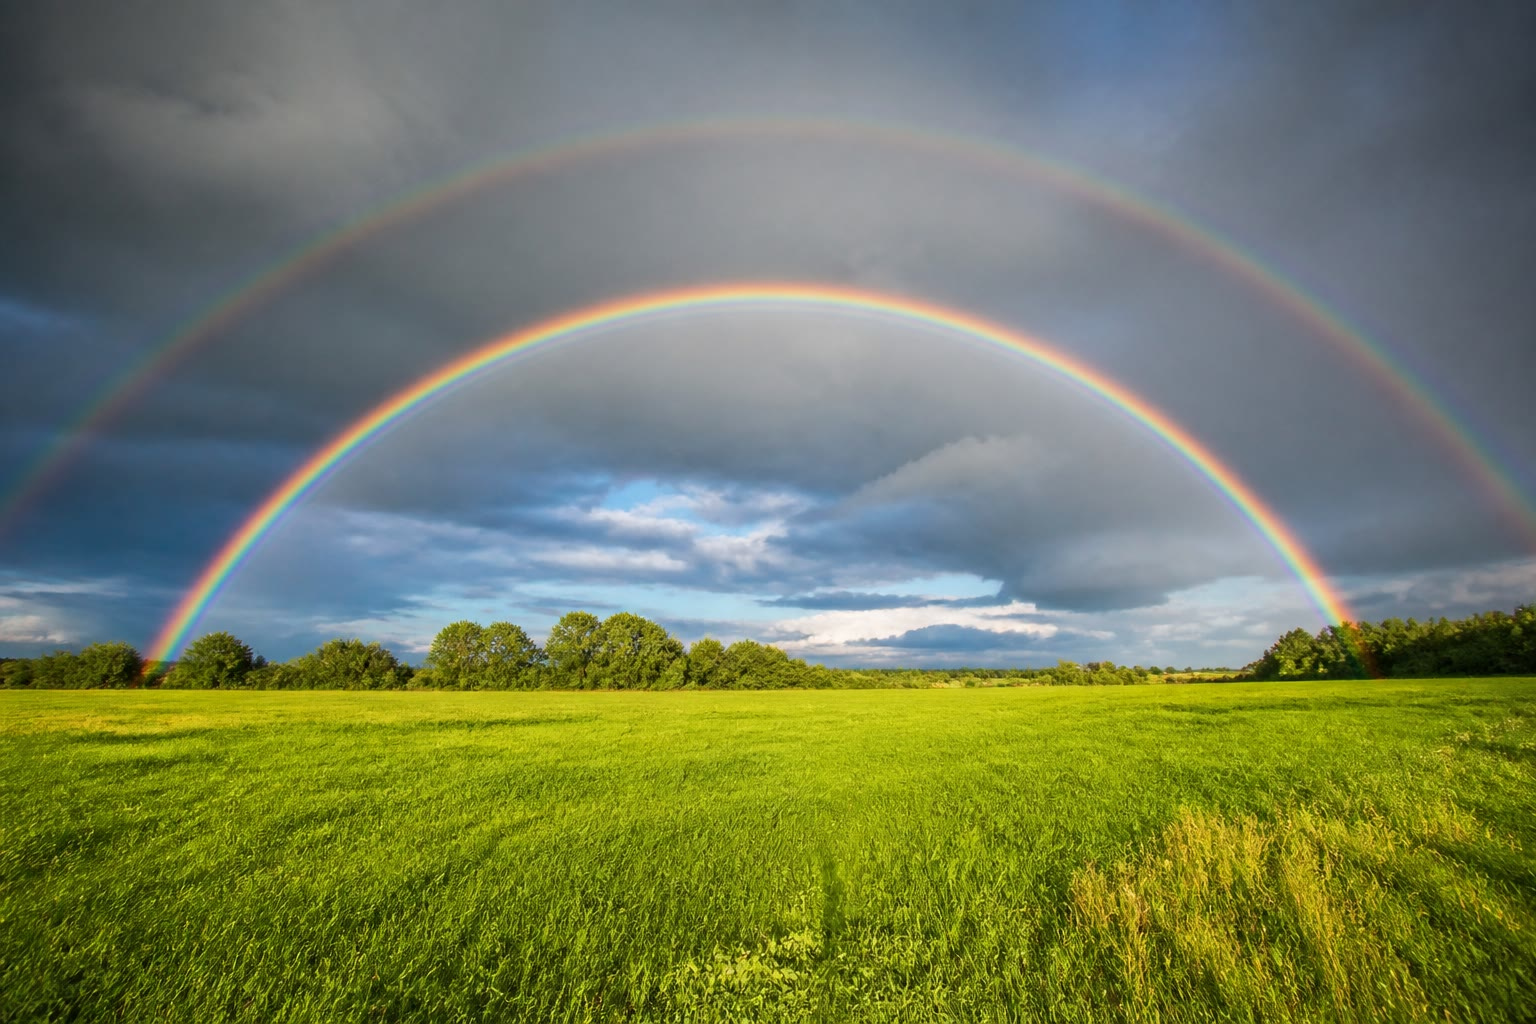
\includegraphics[width=0.60\linewidth]{images/book3/ai/b3-02-rainbow-field.jpg}

{\small Un \omterm{ex:b1:rays-reflection-refraction:rainbow}{arco iris} doble: el arco primario a \qty{42}{\degree} con el rojo por fuera, el secundario, más débil, a \qty{51}{\degree} con los colores invertidos, y la banda oscura de Alejandro entre ambos --- refracción, reflexión y dispersión en cada gota.}
\end{omfigure}

\section{Problema: el enlace de fibra óptica}

\begin{problem}[{Problema de fin de semana --- un hilo de vidrio bajo el
mar: hasta dónde y con qué rapidez puede un pulso de luz llevar un bit
antes de que la geometría, el vidrio y la dispersión lo emborronen}]
\label{pb:b1:rays-reflection-refraction:1}
Un enlace usa una fibra de índice escalonado con \omterm{def:b1:rays-reflection-refraction:fiber}{núcleo} $n_1 = 1.480$,
\omterm{def:b1:rays-reflection-refraction:fiber}{revestimiento} $n_2 = 1.465$, radio del \omterm{def:b1:rays-reflection-refraction:fiber}{núcleo} $a = \qty{25}{\micro m}$, a
la longitud de onda $\lambda_0 = \qty{1550}{nm}$. Dato:
$c = \qty{3.00e8}{m/s}$.

\medskip
\noindent\textbf{Parte I --- La luz en el vidrio.}
\begin{enumerate}
  \item Defínase el índice y calcúlese la velocidad de la luz en el
        \omterm{def:b1:rays-reflection-refraction:fiber}{núcleo}.
  \item ¿Cuánto tarda un pulso en recorrer \qty{50}{km} a lo largo del
        eje?
  \item Calcúlense la frecuencia de la luz y su longitud de onda dentro
        del \omterm{def:b1:rays-reflection-refraction:fiber}{núcleo}.
  \item ¿Por qué se recubre el \omterm{def:b1:rays-reflection-refraction:fiber}{núcleo} con un vidrio de índice menor en vez
        de dejarlo desnudo en el aire, lo que daría un salto de índice
        mayor?
\end{enumerate}

\medskip
\noindent\textbf{Parte II --- El guiado.}
\begin{enumerate}[resume]
  \item Calcúlese el \omterm{thm:b1:rays-reflection-refraction:tir}{ángulo límite} en la superficie núcleo--revestimiento.
  \item Dedúzcase el mayor ángulo que un rayo guiado puede formar con el
        eje.
  \item Un rayo entra por la cara plana desde el aire con un ángulo
        $\theta$ respecto del eje. Muéstrese que queda guiado si
        $\sin\theta \leq
        \sqrt{n_1^2 - n_2^2}$, y calcúlese el \omterm{prop:b1:rays-reflection-refraction:fiber}{ángulo de aceptación}
        $\theta_a$.
  \item Dese la \omterm{def:b1:rays-reflection-refraction:fiber}{apertura numérica}. ¿Por qué un salto de índice mayor
        facilita inyectar luz en la fibra?
  \item La fibra se curva siguiendo un círculo de radio $R_b$. Considérese
        un rayo que viaja paralelo al eje por el borde interior del
        \omterm{def:b1:rays-reflection-refraction:fiber}{núcleo}: muéstrese que alcanza la pared exterior con incidencia $i$
        tal que $\sin i = R_b/(R_b + 2a)$, y hállese el menor $R_b$ para
        el que todavía queda guiado.
\end{enumerate}

\medskip
\noindent\textbf{Parte III --- \omterm{prop:b1:rays-reflection-refraction:fiber}{Dispersión intermodal}.}
\begin{enumerate}[resume]
  \item Exprésense los tiempos de recorrido del rayo axial y del rayo
        guiado más inclinado a lo largo de una longitud $L$.
  \item Dedúzcase el ensanchamiento $\Delta t$ por kilómetro y su valor en
        $L = \qty{2}{km}$.
  \item Un bit es un pulso breve; dos pulsos consecutivos han de quedar
        separados al menos $2\Delta t$ para poder distinguirse. Estímese
        el caudal binario máximo en \qty{2}{km}.
  \item Muéstrese que el producto (caudal binario) $\times$ (longitud) es
        constante para esta fibra, y calcúlese en \unit{Mbit.s^{-1}.km}.
  \item En una fibra de índice gradual el índice disminuye de forma suave
        desde el eje hacia fuera. Explíquese cualitativamente por qué eso
        reduce el ensanchamiento intermodal.
  \item Una fibra monomodo tiene un diámetro de \omterm{def:b1:rays-reflection-refraction:fiber}{núcleo} de unos
        \qty{9}{\micro m}. Compárese con $\lambda_0$ y explíquese por qué
        el modelo de rayos no puede describirla; ¿qué se gana?
\end{enumerate}

\medskip
\noindent\textbf{Parte IV --- Atenuación y dispersión cromática.}
La fibra atenúa la potencia en $\alpha = \qty{0.20}{dB/km}$ a
\qty{1550}{nm}: $P(L) = P_0\,10^{-\alpha L/10}$. El emisor lanza
$P_0 = \qty{1.0}{mW}$; el receptor necesita al menos
$P_{\min} = \qty{1.0}{\micro W}$. Como $n$ depende de $\lambda$, dos
longitudes de onda viajan a velocidades ligeramente distintas: una fuente
de anchura espectral $\Delta\lambda$ da un ensanchamiento del pulso
$\Delta t_c = D\,\Delta\lambda\,L$ con $D = \qty{17}{ps/(nm.km)}$.
\begin{enumerate}[resume]
  \item ¿Qué fracción de la potencia sobrevive a \qty{100}{km}?
  \item Hállese la longitud máxima antes de necesitar un amplificador.
  \item Los amplificadores se colocan cada \qty{100}{km}: ¿qué margen, en
        dB y como cociente de potencias, deja eso para conectores y
        empalmes?
  \item Calcúlese $\Delta t_c$ en \qty{100}{km} para una fuente LED
        ($\Delta\lambda = \qty{40}{nm}$) y para un láser
        ($\Delta\lambda = \qty{0.10}{nm}$); dedúzcase el caudal binario
        máximo de cada una en esa longitud (mismo criterio que antes).
  \item A \qty{850}{nm} la sílice atenúa \qty{2.0}{dB/km}. ¿Qué distancia
        permitiría allí el mismo balance de potencia? ¿Por qué es
        \qty{1550}{nm} la longitud de onda de las telecomunicaciones?
  \item El cable coaxial de cobre atenúa unos \qty{30}{dB/km} a las
        frecuencias necesarias para \qty{1}{Gbit/s}. Compárese la
        separación entre amplificadores con la de la fibra.
\end{enumerate}

\medskip
\noindent\textbf{Parte V --- El enlace completo.}
\begin{enumerate}[resume]
  \item Para la fibra de índice escalonado en \qty{2}{km}, ¿qué efecto
        limita el caudal binario: el ensanchamiento intermodal, el
        cromático (fuente láser) o la atenuación? Dese el caudal binario
        límite.
  \item Para una fibra monomodo en \qty{100}{km} con la fuente láser:
        ¿qué efecto limita y a qué caudal binario?
  \item El enlace monomodo transporta $80$ láseres separados
        \qty{0.8}{nm} en longitud de onda (multiplexación en longitud de
        onda), cada uno al caudal binario de la pregunta anterior.
        ¿Capacidad total?
  \item Fórmese el producto caudal-binario--longitud del enlace de índice
        escalonado y el de un solo canal monomodo; ¿por qué factor gana la
        fibra monomodo y qué único hecho físico lo explica?
\end{enumerate}
\end{problem}
